% % % % % % % % % % % % % % % % % % % % % % % % % % % % % % % % % % % % % % % % % % % %
%                                                                                     %
% Short Sectioned Assignment LaTeX Template Version 1.0 (5/5/12)                      %
% This template has been downloaded from: http://www.LaTeXTemplates.com               %
%                                                                                     %
% Original author:  Frits Wenneker (http://www.howtotex.com)                          %
%                                                                                     %
% Modified by: Fco Javier Sueza Rodríguez (fcosueza@disroot.org)                      %
%                                                                                     %
% Changes:                                                                            %
%	    - Custom Chapters, Sections and Subsections (titlesec package)                %
%           - Document type scrbook (oneside)                                         %
%           - Use babel-lang-spanish package and marvosym                             %
%           - Use hyperref, enumitem, tcolorbox and glossaries packages               %
%           - Use Time New Roman (mathptmx), Helvetic and Courier fonts               %
%                                                                                     %
% License: CC BY-NC-SA 3.0 (http://creativecommons.org/licenses/by-nc-sa/3.0/)        %
%                                                                                     %
% % % % % % % % % % % % % % % % % % % % % % % % % % % % % % % % % % % % % % % % % % % %

%-----------------------------------------------%
%	              Packages                  %
%-----------------------------------------------%

\documentclass[paper=a4, fontsize=11pt, oneside]{scrbook}

% ---- Text Input/Output ----- %

\usepackage[T1]{fontenc}
\usepackage[utf8]{inputenc}
\usepackage{mathptmx}
\usepackage[scaled=.92]{helvet}
\usepackage{courier}
\usepackage[indent=12pt]{parskip}

\usepackage{geometry}
\geometry{verbose,tmargin=3cm,bmargin=3cm,lmargin=2.6cm,rmargin=2.6cm}

% ---- Language ----- %

\usepackage[spanish]{babel}
\usepackage{marvosym}

% ---- Another packages ---- %

\usepackage{amsmath,amsfonts,amsthm}
\usepackage{graphics,graphicx}
\usepackage{titlesec}
\usepackage{fancyhdr}
\usepackage{tcolorbox}
\usepackage{hyperref}
\usepackage{enumitem}
\usepackage[automake]{glossaries}

%--------------------------------------------------------------------%
%                      Customizing Document                          %
%--------------------------------------------------------------------%


% ----------- Custom Chapters, Sections and Subsections -------------- %

\titleformat{\chapter}[display]
			{\bfseries\Huge}
			{Tema \ \thechapter} {0.5ex}
			{\vspace{1ex}\centering}

\titleformat{\section}[hang]
			{\bfseries\Large}
			{\thesection}{0.5em}{}

\titleformat{\subsection}[hang]
			{\bfseries\large}
			{\thesubsection}{0.5em}{}

\titleformat{\subsubsection}[hang]
			{\bfseries\large}
			{\thesubsubsection}{0.5em}{}

\hypersetup{
    colorlinks=true,
    linkcolor=black,
    urlcolor=magenta
}

% ------------------- Custom heaaders and footers ------------------- %

\pagestyle{fancyplain}

\fancyhead[]{}
\fancyfoot[L]{}
\fancyfoot[C]{}
\fancyfoot[R]{\thepage}

\renewcommand{\headrulewidth}{0pt} % Remove header underlines
\renewcommand{\footrulewidth}{0pt} % Remove footer underlines

\setlength{\headheight}{13.6pt} % Customize the height of the header

% --------- Numbering equations, figures and tables ----------------- %

\numberwithin{equation}{section} % Number equations within sections
\numberwithin{figure}{section} % Number figures within sections
\numberwithin{table}{section} % Number tables within sections

% ------------------------ New Commands ----------------------------- %

\newcommand{\horrule}[1]{\rule{\linewidth}{#1}} % Create horizontal rule command


%----------------------------------------------------------------------------------------
%	TÍTULO Y DATOS DEL ALUMNO
%----------------------------------------------------------------------------------------

\title{
\vspace{10ex}
\normalfont \normalsize
\huge \textbf{Manual de Estilo: Web AdminSys}
}
\author{Francisco Javier Sueza Rodríguez}
\date{\normalsize\today}

%----------------------------------------------------------------------------------------
%                                     DOCUMENTO
%----------------------------------------------------------------------------------------
\begin{document}

\maketitle

\thispagestyle{empty}

\vspace{75ex}

\begin{center}
    \begin{tabular}{l l}
        \textbf{Centro}: & IES Aguadulce \\
        \textbf{Ciclo Formativo}: & Desarrollo Aplicaciones Web (Distancia)\\
        \textbf{Asignatura}: & Diseño de Interfaces Web\\
        \textbf{Tema}: & Tema 2 -  Hojas de Estilo\\
    \end{tabular}
\end{center}

\newpage

\tableofcontents

\vspace{20ex}

\hrule

\vspace{18ex}

\listoffigures

\newpage

\section{Bocetos}
En este apartado se van a mostrar bocetos de la página web de la empresa \textit{\textbf{AdminSys}}. Se han realizado dos bocetos, un \textbf{boceto no detallado} de la página completa y un \textbf{boceto detallado} del pie de página.

\subsection{Boceto No Detallado (Página Completa)}

En el \textbf{boceto no detallado} podemos ver las principales secciones de la página. En este boceto no se va a incluir texto ni imagen alguna, solo es un esbozo de las diferentes secciones que componente la página.

La página tendrá una \textbf{cabecera} divida en 3 subsecciones debajo de esta y a la derecha en un elemento aside encontramos el \textbf{menú de navegación}. Debajo de la cabecera y a la izquierda del menú tenemos la \textbf{sección de contenido}, dividida en dos subsecciones con diferentes contenido. Por último, tenemos el \textbf{pie de página}, que se encuentra debajo del resto de secciones.

En la siguiente imagen vemos el boceto de la página web principal.

\begin{figure}[H]
    \centering
    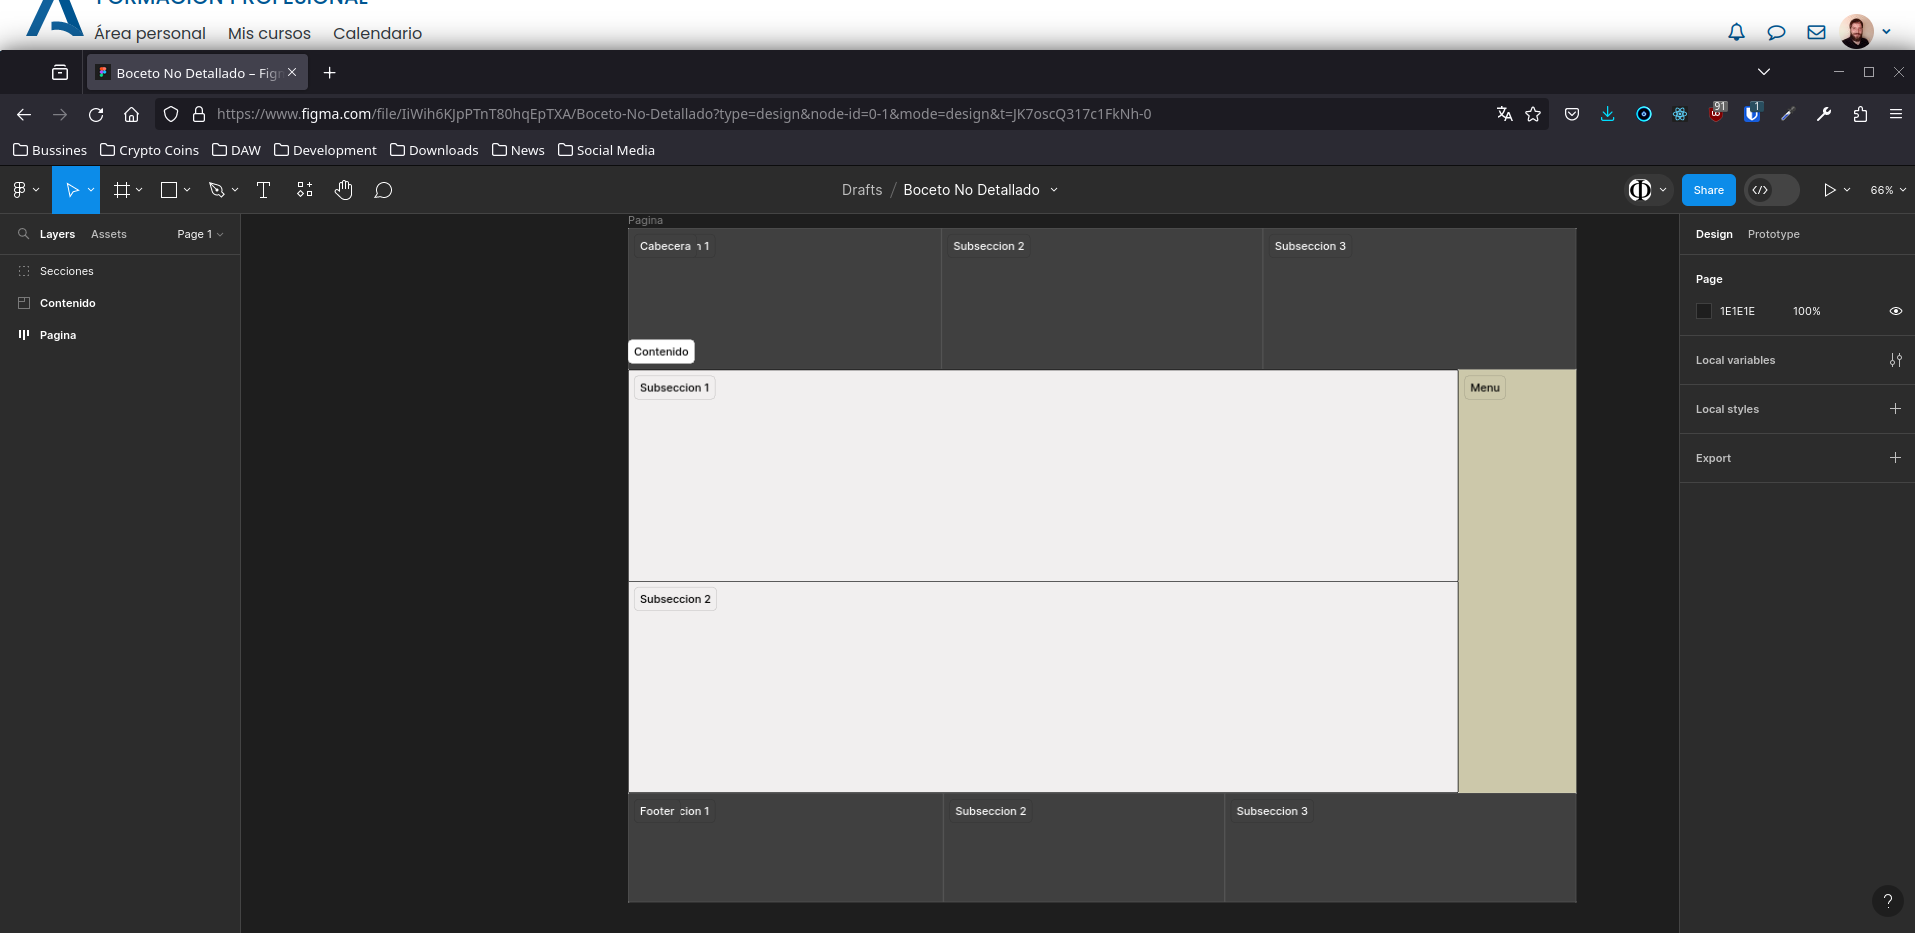
\includegraphics[scale=0.30]{boceto-pagina.png}
    \caption{Imagen del boceto de la página completa}
\end{figure}

\subsection{Boceto Detallado (Pie de Página)}

En segundo lugar se ha realizado un \textbf{boceto detallado} del pie de página, donde podemos observar 3 subsecciones diferentes. En este boceto si se van a incluir tanto los textos como los iconos que se van a emplear en el pie de página. No se ha empleado texto ni imágenes placeholder, sino que se ha usado el texto e imágenes definitivas.

En la \textbf{primera sección} se muestra un formulario con 3 elementos checkbox donde el usuario podrá seleccionar que políticas de cookies aplicar. En la \textbf{segunda} sección tenemos un pequeño menú con entradas acerca de información relacionada con la empresa, estas son \textbf{Soporte}, \textbf{Política de Privacidad} y \textbf{Acerca de}. En la \textbf{última sección} tenemos varios iconos con enlaces a las redes sociales donde tiene presencia la empresa.

En la siguiente imagen podemos ver el boceto con detalle.
\begin{figure}[H]
    \centering
    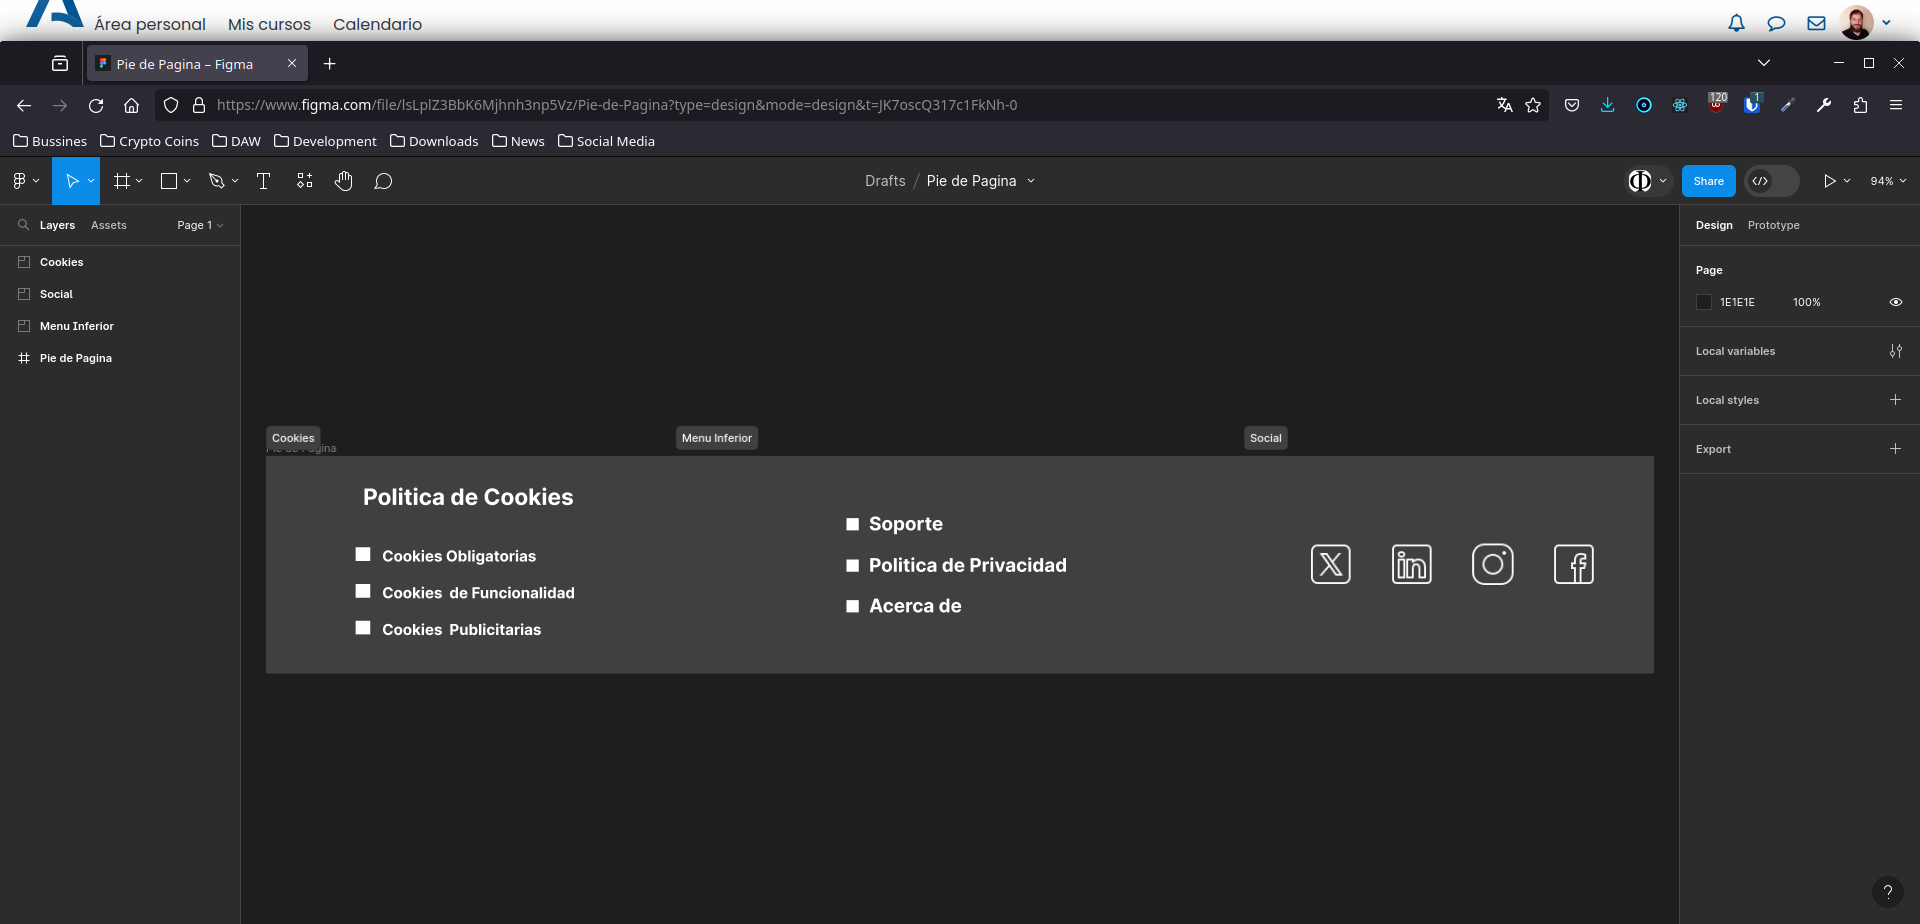
\includegraphics[scale=0.30]{boceto-pie.png}
    \caption{Imagen del boceto de pie de página}
\end{figure}

\section{Colores y Fuentes}
En esta sección del manual se va a especificar la paleta de colores seleccionada y en que elementos se va a emplear cada color, así como una descripción de las fuentes que se van a usar en la página web.

\subsection{Paleta de Colores}
La paleta de colores elegida ha sido una escala de grises, para darle un toque corporativo y serio a la web. Los colores que se han usado los podemos ver en la siguiente imagen.

\begin{figure}[H]
    \centering
    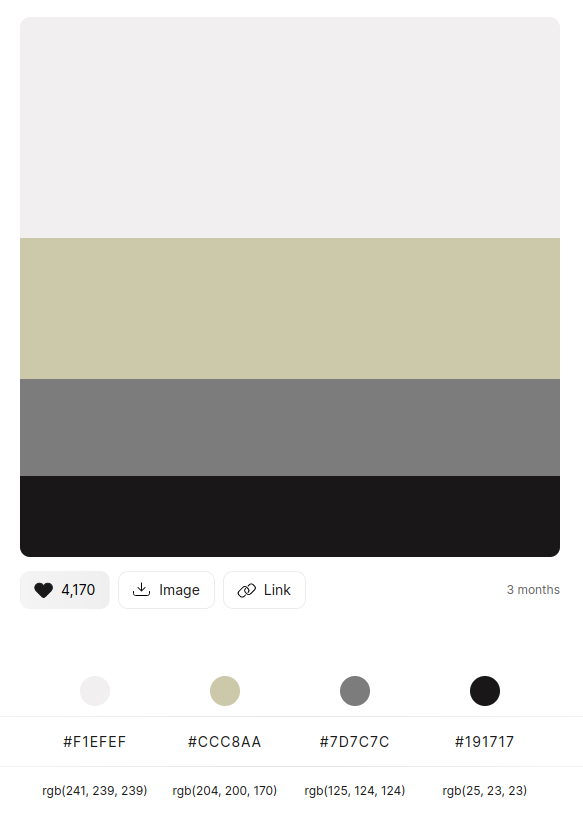
\includegraphics[scale=0.40]{paleta-de-colores.png}
    \caption{Paleta de colores empleada}
\end{figure}

Los colores se han usado de la siguiente manera:

\begin{itemize}
    \item \textbf{Blanco} (\textbf{\textit{rgb(241, 239, 239)}}): se ha usado para la sección de contenido, además de para el color de la fuente de la cabecera y el pie de página. Es el color principal de la web.

    \item \textbf{Negro} (\textbf{\textit{rgb(25, 23, 23)}}): el negro se ha usado para el fondo de la cabecera y el pie de página. En este caso, se le ha aplicado una ligera transparencia para rebajar un poco el color y que sea un poco menos oscuro. También se ha empleado para el color de la fuente del menú y del contenido, en este caso, sin aplicar transparencia, ya que nos interesa que haya más contraste.

    \item \textbf{Gris Claro} (\textbf{\textit{rgb(204, 200, 170)}}): este gris se ha utilizado para el fondo del menú de navegación.

    \item \textbf{Gris Oscuro} (\textbf{\textit{rgb(125, 124, 124)}}): este tono de gris se ha utilizado para resaltar algunos elementos, como los botones.
\end{itemize}

Se han definido variables en el fichero CSS, tanto de la maqueta como el principal, para facilitar el uso de los colores. En la siguiente imagen, se muestra la definición de las variables en el editor VS Code.

\begin{figure}[H]
    \centering
    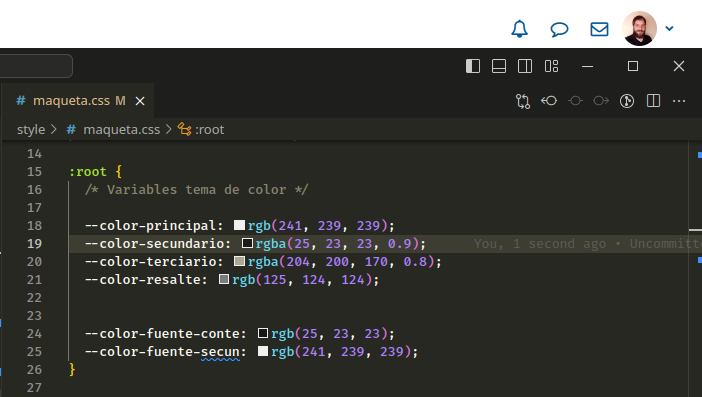
\includegraphics[scale=0.70]{variables-css.png}
    \caption{Declaración de variables CSS}
\end{figure}

\subsection{Fuentes}
Para el desarrollo de la página web se han seleccionado dos tipos de fuentes diferentes, aunque pertenecen a la misma familia. Las fuentes seleccionadas han sido \href{https://fonts.google.com/specimen/Roboto}{Roboto} y \href{https://fonts.google.com/specimen/Roboto+Slab?query=robot+slab}{Roboto Slab}.

La primera de ellas, \textbf{Roboto}, es una fuente \textbf{sans-serif} que vamos a emplear para la mayoría de textos que hay en la página web, ya que al ser sans-serif será más cómoda su lectura.

Por otro lado, para los títulos y el nombre de la empresa se ha seleccionado \textbf{Roboto Slab}, de la misma familia que Roboto pero está es \textbf{serif}, ya que este tipo de fuentes dan un toque más estilizado y visual al texto, por lo que es apropiada para textos cortos y que tienen que resaltar.

En la siguiente captura, una realizada a la sección de noticias de la web, se puede ver el empleo de ambas fuentes, una en el título de la noticia (Roboto Slab) y otra en su cuerpo (Roboto).

\begin{figure}[H]
    \centering
    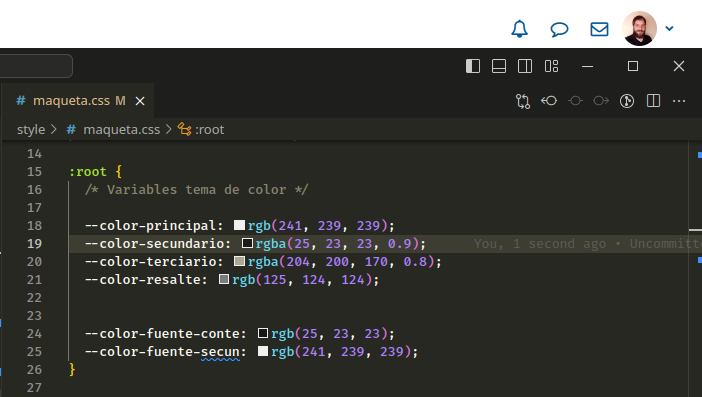
\includegraphics[scale=0.70]{variables-css.png}
    \caption{Uso de las fuentes en la web}
\end{figure}

\section{Maquetas}
En ese apartado se han realizado dos maquetas de la web. Una de ellas sobre la \textbf{página web completa} empleando \textbf{CSS Grid} y otra más detallada del \textbf{pie de página} empleando \textbf{CSS Flex}.

\subsection{Maqueta Página Completa}
Se ha realizado una maqueta de la página principal usando \textbf{CSS Grid}. En este caso, se ha decidido aplicar CSS Grid a un div que contiene a todos los elementos de la página, para posicionar los \textbf{elementos principales}, en este caso, header, aside, main, y footer. Se ha realizado así para mantener la estructura de la página más simple, usando flexbox dentro de los elementos para posicionar las subsecciones.

En la parte de la \textbf{cabecera} no se han incluido el logo o la imagen que va a llevar la versión definitiva, por lo que puede ser que su tamaño varíe ligeramente para acomodar bien las fotos y que no se vea demasiado amontonado. En la siguiente imagen, se puede ver una captura de esta maqueta.

\begin{figure}[H]
    \centering
    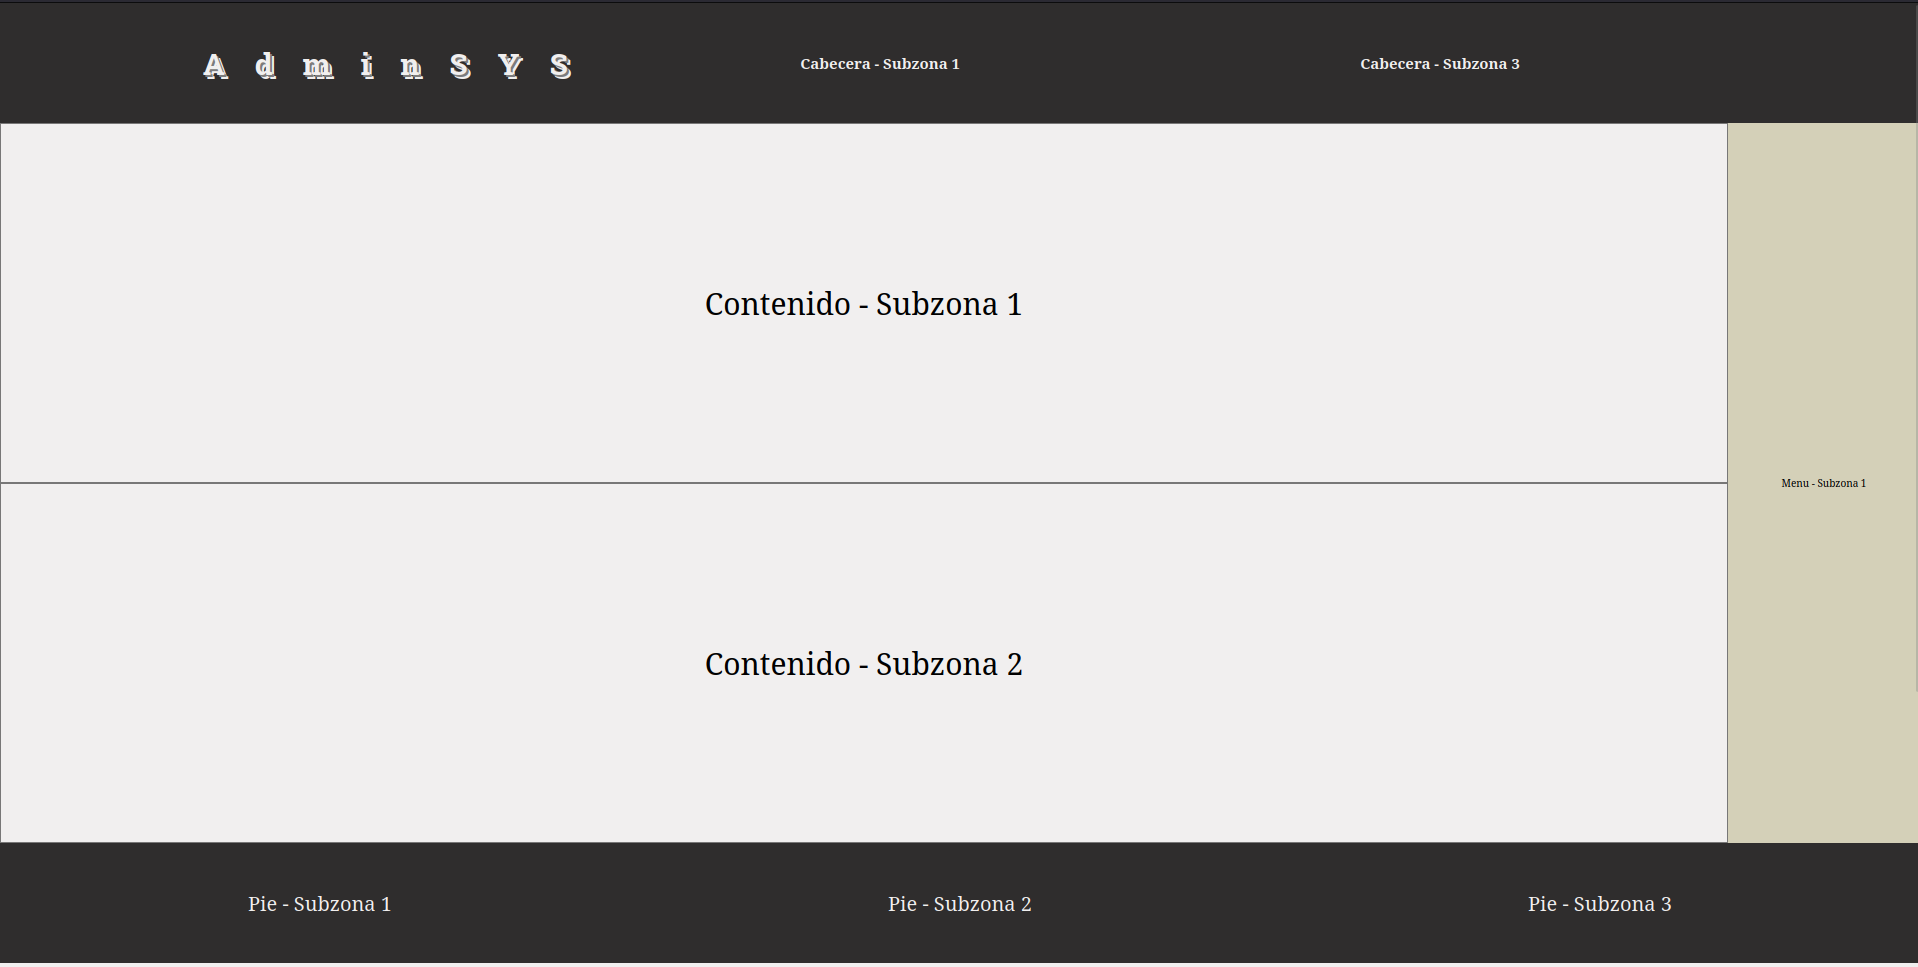
\includegraphics[scale=0.23]{maqueta-pagina.png}
    \caption{Maqueta página completa}
\end{figure}

Hay algunos detalles que \textbf{se han incluido} por \textbf{requerimientos de la tarea}, pero que por razones estéticas y de legibilidad \textbf{se excluirán en la versión final}, en este caso, la sombra aplicada al texto con el nombre de la empresa no se implementará en la versión final, ya que dificultad la legibilidad del texto.

\subsection{Maqueta del Pie de Página}
La maqueta del \textbf{pide de página} se ha realizado utilizando  \textbf{CSS Flex}, en el contenedor principal, estos es, la etiqueta \textbf{footer}, y empleando flex-grow para que los 3 elementos tengan el mismo tamaño. Dentro de cada elemento se ha usado justify-content y align-items, para centrar los elementos en la posición deseada. En la siguiente imagen podemos ver una captura de la maqueta del pie de página.

\begin{figure}[H]
    \centering
    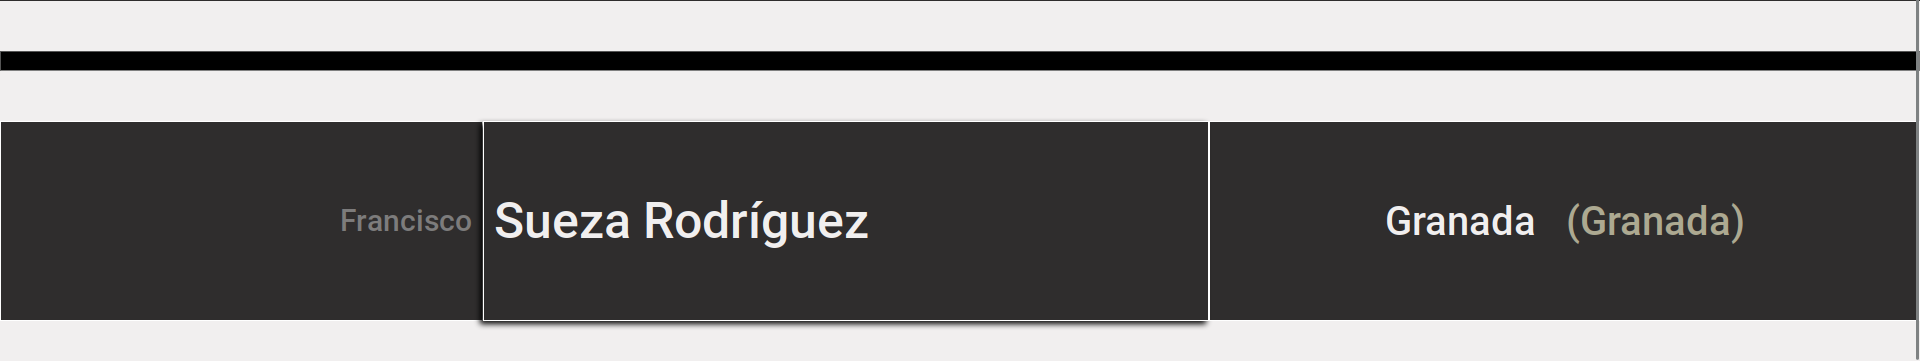
\includegraphics[scale=0.23]{maqueta-pie.png}
    \caption{Maqueta pie de página}
\end{figure}





% Bibliography

%\newpage
%\bibliography{citas}
%\bibliographystyle{unsrt}

\end{document}